\documentclass[review]{elsarticle}

\usepackage{lineno,hyperref}

\usepackage{geometry}
\usepackage{qtree}

\usepackage[]{algorithm2e}
\usepackage{amsthm}
\newtheorem{theorem}{Theorem}[section]
\newtheorem{corollary}{Corollary}[theorem]
\newtheorem{example}{Example}
\newtheorem{lemma}[theorem]{Lemma}
\usepackage{rotating}
\usepackage[utf8]{inputenc}
\usepackage[T1]{fontenc}    % use 8-bit T1 fonts
\usepackage{lmodern}
\usepackage{hyperref}       % hyperlinks
\usepackage{lipsum}

\usepackage{color, colortbl}

\definecolor{Gray}{gray}{0.9}
\definecolor{goldenpoppy}{rgb}{0.99, 0.76, 0.0}
\definecolor{goldenrod}{rgb}{0.85, 0.65, 0.13}

\usepackage[protrusion=true,expansion=true]{microtype}

\usepackage{amssymb}
\usepackage{amsfonts}
\usepackage{booktabs}
\usepackage{eqnarray,amsmath}
\usepackage[table]{xcolor}

\usepackage{listings}
\usepackage{dirtytalk}

\usepackage{rotating}
\usepackage{caption}

\usepackage{graphics}

\usepackage{graphicx}


\usepackage{indentfirst}
\usepackage[utf8]{inputenc}
 \usepackage{subcaption}

 
\usepackage{xspace,color}
\usepackage{url}

\usepackage[export]{adjustbox}

\usepackage{listings}
\usepackage{xcolor}

\modulolinenumbers[5]

\journal{Journal of \LaTeX\ Templates}

%%%%%%%%%%%%%%%%%%%%%%%
%% Elsevier bibliography styles
%%%%%%%%%%%%%%%%%%%%%%%
%% To change the style, put a % in front of the second line of the current style and
%% remove the % from the second line of the style you would like to use.
%%%%%%%%%%%%%%%%%%%%%%%

%% Numbered
%\bibliographystyle{model1-num-names}

%% Numbered without titles
%\bibliographystyle{model1a-num-names}

%% Harvard
%\bibliographystyle{model2-names.bst}\biboptions{authoryear}

%% Vancouver numbered
%\usepackage{numcompress}\bibliographystyle{model3-num-names}

%% Vancouver name/year
%\usepackage{numcompress}\bibliographystyle{model4-names}\biboptions{authoryear}

%% APA style
%\bibliographystyle{model5-names}\biboptions{authoryear}

%% AMA style
%\usepackage{numcompress}\bibliographystyle{model6-num-names}

%% `Elsevier LaTeX' style
\bibliographystyle{elsarticle-num}
%%%%%%%%%%%%%%%%%%%%%%%

\begin{document}

\begin{frontmatter}

\title{Use law of large numbers to measure Neural Networks optimizers performance\tnoteref{mytitlenote}}
\tnotetext[mytitlenote]{.}

%% Group authors per affiliation:
\author{Mayra Cristina Berrones Reyes\fnref{myfootnote}}
\address{Universidad Aut\'onoma de Nuevo Le\'on. Facultad de Ingenier\'ia Mec\'anica y El\'ectrica}
\fntext[myfootnote]{San Nicol\'as de los Garza, Nuevo Le\'on. M\'exico.}


\begin{abstract}
In this work, we want to explore some of the qualities of different optimizers used in training Neural Networks. With the Law of Large Numbers we want to see if the optimizers are affected in a good or a bad way when given more iterations of training. If it helps them converge to the highest average of accuracy percentage, or if in some cases it becomes flawed and lands in over training. 

\end{abstract}

\begin{keyword}
Neural Networks \sep Statistics \sep Optimizers \sep Law of Large Numbers 
\MSC[2020] 00-01\sep  99-00
\end{keyword}

\end{frontmatter}

\linenumbers

\section{Introduction}\label{introduction}

In the subject of problem solving and finding an optimal solution to issues we encounter in our day to day lives, a popular item is the topics of Machine Learning (ML) and Artificial Intelligence (AI), which mainly promises to find a faster and acceptable solution. Some of this methods, however, rely heavily on a random factor, that allow them to sometimes find an answer faster than in the case of traditional statistical methods.\\

So the question becomes here, is there a difference between statistics and ML? In this case, the answer can be that they are certainly similar in some aspects, as the two fields are converging more and more in different subjects, for example, both ML and statistics are used nowadays on techniques of pattern recognition, data mining, knowledge discovery, etc. \\

Defining them separately, we have that ML is a sub field of computer science. It concentrates on building systems that can learn from data, instead of relaying on explicit instruction of programs. A statistical model on the other hand has a more mathematical background. The main difference between the two is that ML focuses on optimization, performance and finding generalizable predictive patterns while statistics is more concerned with the inferences it can make from a sample of the population \cite{wstat}.\\

For a ML model, any prior assumptions about the underlying relationships between the variables we are studying are not needed in order to start building your model. In some instances, we can just give all of the data we have, and the algorithm can process the data and find patterns in it. Up until a few years back, all the process and calculations that the algorithm of ML made in its way to learn and find a suitable answer where treated as a \textit{black box}, with a mentality that, as long as it works, we do not have to concern ourselves with how it got to the final result.\\

This practice stoped being acceptable when more and more scientist wanted to use models based on ML and AI to solve real life problems, but got rejected because they could not prove with detail why their model worked the way it did. In direct contrast, in the field of statistics first we need to collect and understand certain features of the data we are working with. How it was collected, the statistical properties, the distribution of the population we are using, etc. \\

Here we find another difference between these two fields. Generally speaking, ML modeling thrives on high dimensional data sets. The more data you give your model, the more accurate your prediction ends up being. In the case of statistical modeling, they are usually applied on low dimensional data sets.\\

In a comprehensive comparison between these two fields \cite{kdnuggets1} we find an example of the main difference at interpreting results from each model in List \ref{ls1}. In this example we see that statistical models offer a better chance at reproducibility of the experiments than the models of ML. This is a highly valued feature when publishing an article of these sort of investigations.\\

\begin{itemize} \label{ls1}
\item \textbf{Machine Learning model:} \say{The model is 85\% accurate in predicting Y, given \textit{a}, \textit{b} and \textit{c}.}
\item \textbf{Statistical model:} \say{The model is 85\% accurate in predicting Y given \textit{a}, \textit{b} and \textit{c}, and I am 90\% certain that you will obtain the same results.}
\end{itemize}

Overall, regarding all of these points, it may seem that ML and statistical modeling are two separate branches of predictive techniques. These differences however, have been reduced significantly over the last decade, where statistical models have adopted some methods from machine learning, creating an emerging field called statistical learning. ML in return tries to implement statistical strategies to justify the behavior of the model, its results, and dispel the idea of the \textit{black box} when it comes to the calculations of the model.\\

Following the idea of these two fields working together, in this work we take a closer look at one of the most popular uses of ML modeling, which is Neural Networks (NN) and its derivates. %Using some techniques from statistical methods we are going to evaluate the use of certain features in the NN such as how can we choose the best optimizer for our model before we begin the computational costly process of training.\\

\section{Background}\label{background}

As mentioned in the Introduction section \ref{introduction} the main goal for this article is to approach a machine learning issue with a statistical set of mind, and see if we are able to arrive to a reasonable answer. In this case, we have a theoretical problem for a machine learning algorithm known as Convolutional Neural Network (CNN).  \\

In previous works \cite{tesis} (article in revision) we have worked with a self made architecture of a CNN model that will help us classify medical images of mammograms, and help medical professionals unload their pre processing work by labeling the data of images with and without anomalies. In this works, we trained and modeled about 200 different architectures, changing parameters such as optimizers, size of the image, number of neurons, number of hidden layers, etc.\\

Finishing all of those experimentations with the different parameters of the CNN took us almost a whole year, even with the use of powerful hardware, and parallel programing. At the end of the experimentation, we concluded that one of the most important feature that helped us determine which model architecture worked better was the optimizer we used. Adam and SGD where the more robust, having all of their models at a steady percentage of accuracy above the 95\%, and Adadelta was the one that had two of the models with best accuracy out of all of them.\\

Part of the training process of a NN model is to change some of the wights to try to minimize our loss function and maximize the accuracy of our predictions. This is where the optimizers come in. They help with the update of parameters in response to the loss function, and depending on the type of optimizer we choose, it determines how big the changes must be in each iteration. This is known as a learning rate. We now have a brief introduction to each of the three optimizers that we are working on this article. (For a more in depth explanation we suggest the following articles \cite{adam} \cite{adadelta} \cite{sgd}) \\

\subsection{SGD}
We begin by discussing the SGD optimizer, since it is one of the oldest approaches to an optimization algorithm. It stands for stochastic gradient descent.  Starting form a initial value, this algorithm runs iteratively to find the optimal value given by the cost function. It is very simple, but perhaps for its simplicity, it finds several problems, for example, compared to other optimizers, it converges at a slower rate. It also has problems with being stuck in a local minimum. Newer approaches have outperformed SGD in optimizing the cost function, so some boosters have been implemented to correct its disadvantages, like momentum \cite{momentum}, nesterov \cite{nesterov} or a combination of both.\\
\subsection{Adam}

Adam stands for adaptive moment estimation. It is one of the most popular optimizers used in machine learning, as it is the one that performs best on average. It uses the same concept of the SGD plus momentum and adaptive learning rates to converge faster to the optimal value. The concept of adaptive learning rates can be pictured as a match of golf. We are allowed to move faster initially, but as the learning rate decays, we take smaller and smaller steps, allowing a fast convergence, since there is less chance of overstepping our goal.\\

\subsection{Adadelta}

Now with Adadelta, we can say that it is like a progression of the previous optimizers. As Adam, this is an algorithm based in an adaptive learning rate. It more closely resembles Adagrad (another optimizer of the same distribution as Adam) and in this case, it seeks to reduce the aggressive decreasing learning rate. Compared with all the other optimizers, Adadelta is the one that seems to converge the fastest, as shown in Figure \ref{fig1}.\\


\begin{figure}[]
  \centering
  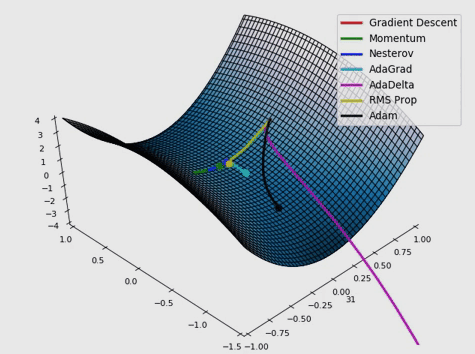
\includegraphics[width=.7\linewidth]{optimizers.png}  
	\caption{Comparison of other optimizers \cite{opti}}
\label{fig1}
\end{figure}

Selecting this three optimizer we continued to do experiments with the other parameters of the CNN that we could change. An important distinction was that, for all of the changeable parameters we had, we stablished some that remained fixed for the entire experiment. One of these parameters was the number of iterations and epochs we used to train all the models. In our case we had 10,000 small iterations, and 10 epochs (large iterations). For the validation set we had 2,000 small iterations. \\

A quick way to explain the difference between these mentioned small and large iterations is as follows. In the first epoch or large iteration, we train our model with 10,000 small iterations. At the end of this first epoch, the model is expected to have a small percentage in accuracy, and when the small iterations end, the model is tested against the developing set for 2,000 small iterations. This helps the model modify some of its weights in preparation for the next epoch. When all of the epochs end, the model has finished its training, and it is expected that the resulting accuracy percentage closely resembles the accuracy we will get when we use the model on the test set.\\

When we made the comparison of these three optimizers we found that, for some models of the Adam and Adadelta optimizers, their performance on the test set was not consistent with the result on their training, while in the case of the optimizer SGD all of their accuracy remained in a steady range. Robustness in a model and reproducibility is something well sought out by researchers, and SGD provided that for our models. However, none of the models ever reached an accuracy percentage above of 96\%. Doing a thorough scan of the behavior of all of the models from these three optimizers we realized that Adam and Adadelta reach a high accuracy percentage by the eighth epoch of training, and all the accuracy achieved after that comes in very small intervals.\\

In contrast, we saw that the models with a SGD optimizers had a very slow climb of their percentage accuracy, but it continued its constant pace, til it ends in the tenth epoch (as all the other models). This behavior made us believe that, if we gave more iterations to these models, than the accuracy will improve, and maybe even surpass the accuracy of all other models eventually.\\

This can also be said in favor of the other two optimizers, so, in order to compare fairly these experimentation, we will need to reach a point in which there is no discernible improvement in the performance of any of the optimizers, and see if they average to an accuracy above that of what we registered so far.\\

The problem now is that we do not have the time or the computational resources to do an experimentation of that scale with the same dataset, specially with the amount of epochs we are trying to achieve, so in this experiment we will be using a toy dataset of images of cats and dogs, which can come close to the binary experimentation we used for out previous models. In the next section we see a brief explanation of the inner workings of our experiment, and a discussion of some statistical themes that will help us strengthen our results.\\

\subsection{Law of large numbers}
The idea behind this experiment, comes with the basis of the Law of Large Numbers (LLN). The LLN states that if you repeat an experiment a large number of times, averaging the results, then your answer should be as close as the expected value. In Theorem \ref{lln} we see the common notation for the sample mean \cite{lawln}.\\

\begin{theorem}[\textbf{Law of Large Numbers}]
\label{lln}
For i.i.d. random variables $X_1$, $X_2$, $...$, $X_n$ the sample mean, denoted by $\overline{X}$, is defined as
\[\overline{X} = \frac{X_1+ X_2 + ... + X_n}{n}\]
Another common notation for the sample mean is $M_n$. If the $X_i$s have CDF $F_x(x)$, we might show the sample mean by $M_n(X)$ to indicate the distribution of the $X_i$s.
\end{theorem}
\begin{flushright}
$\blacksquare$
\end{flushright}

Since we have that the LLN often deals with any sort of trial with a probabilistic outcome, the application in our case becomes clearer. Machine learning systems, such as a CNN adapt very quickly to a large amount of data being feed into it. The data entries will in this case represent the trials, and the resulting average of accuracy of the training process are the patterns and features that the CNN has to make a classification. \\

The basic nature of the learning process of the CNN is exactly what the LLN represents as a mathematical approach, only translated to a more operational format. In other words, the process of each epoch in our model can translate loosely at what the LLN represents. So in this experiment we give all three optimizers the chance to even out their learning rate by giving them more iterations to train the data \cite{sirignano}.\\


\section{Methods and materials}\label{method}

As we stablished in the Background section, there are many parameters in a CNN that can be tuned to try to improve the performance of our model. The main propose of this experiment is to establish if it is worth it to spend the time and computational processing to give more epochs to the models, to see if they can reach a higher accuracy percentage. We test this hypothesis  with a toy data set of images of dogs and cats, and pre trained weights pulled from the ResNet50 neural network to accelerate the training process.\\

All of the experimentation was carried out in a Google Colab notebook, in a MacBook Pro 13-inch 2016.\\

\subsection{Dataset and models}

For the experiment we are using a dataset consisting on images of cats and dogs. The data sets are divided by 23,000 images on the training set, 2,000 images for the validation or developing set, and lastly 12,500 images for the test set. In Figure \ref{fig2} we have an example of some of the images of our toy dataset. The resolution of all of them is kept at 150$\times$150 pixels.

\begin{figure}[]
  \centering
  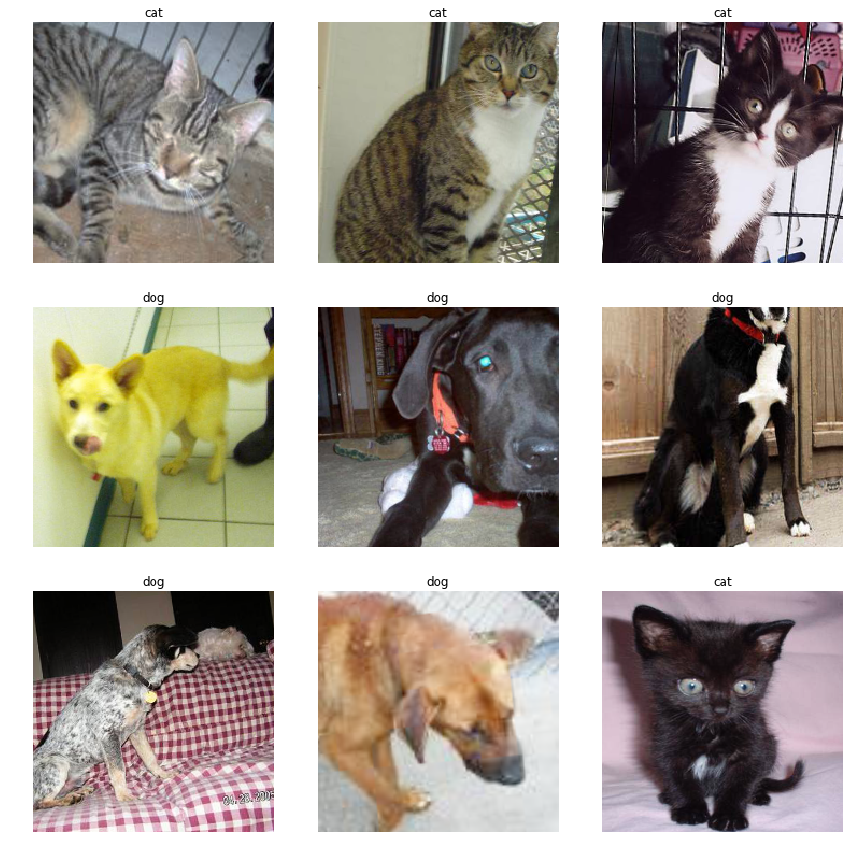
\includegraphics[width=.6\linewidth]{cats.png}  
	\caption{Example of some of the images on our dataset}
\label{fig2}
\end{figure}

The libraries used on the experiment we have Keras, Matplotlib, sklearn and h5py.\\

We mentioned before that, in order to keep the time of the training process as minimal as possible, we began with pre trained weights of the ResNet50 using as input imagenet \footnote{Repository with experimentation. \url{https://github.com/mayraberrones94/Probabilidad/blob/master/ProyectoFinal/Code/Elisa_Exp.ipynb}}. We then assigned the paths to the different datasets, and added some image augmentation by using the data generator that the library Keras has installed.\\

As discussed in previous sections, we are giving the models more iterations to train. In this case we have 300 epochs for each model. We add a restriction to each epoch instead of small iterations, that monitors the loss function, and when it detects that there is no improvement for more than 5 iterations, with a slope of 0.02 on the learning rate, gives a break and passes to the next epoch. This is a common practice to avoid overfitting your model.\\

\section{Experiments with Adam, Adadelta and SGD}
 
 In Figure \ref{fig3} we see the accuracy performance of the training set. We can appreciate the same feature explained in the Background section, in which thanks to the adaptive learning rate, the optimizers Adam and Adadelta move to a very high accuracy since the first epochs, and slowly even out to a more horizontal behavior. Still, it is barely visible, but comparing these two we see that, despite the little bumps along the line to the 300 epoch, the Adam optimizer is still climbing the accuracy. \\
 
 In the case of the SGD optimizer, as we predicted, the curve does not even out until more than half of the epochs have passed. Again, it is almost imperceptible because of the little bumps, but we can see that the line has a small tendency of going upward.\\
 
 
\begin{figure}[]
  \centering
  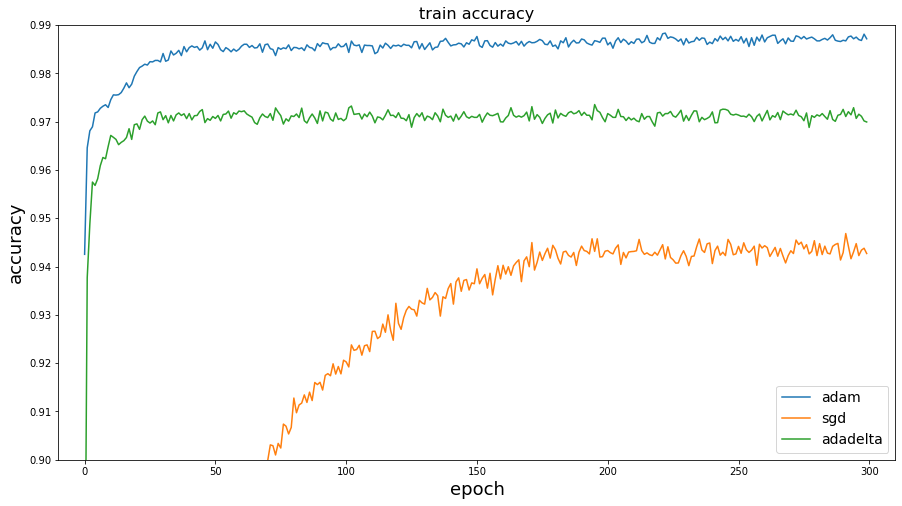
\includegraphics[width=.9\linewidth]{trainacc1.png}  
	\caption{Plot of the accuracy of the models after 300 epochs in the training dataset}
\label{fig3}
\end{figure}

In Figure \ref{fig4} we have the accuracy of the validation set. In this case, for the Adadelta and the SGD optimizers we do reach a line where no improvement is made throughout the rest of the epochs. Adadelta reaches it in roughly the same time that in Figure \ref{fig3} the curve evens out. These two optimizers also improved their accuracy in comparison with the training.\\

In the Adam optimizer, the spikes on the line become more prominent than in the training, and when it finally evens out on the last epochs, we can see that it does not reach the same accuracy as the training.\\

\begin{figure}[]
  \centering
  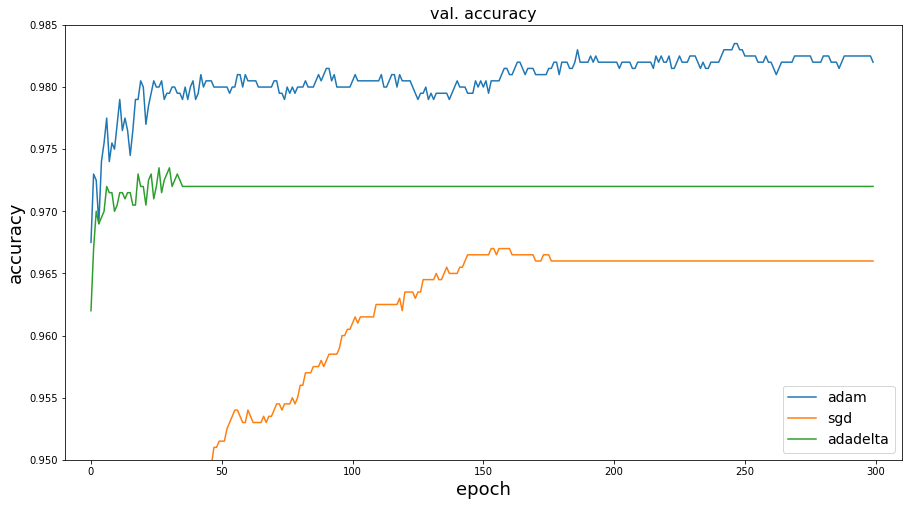
\includegraphics[width=.9\linewidth]{valacc1.png}  
	\caption{Plot of the accuracy of the models after 300 epochs in the validation dataset}
\label{fig4}
\end{figure}

In Figure \ref{fig5} and \ref{fig6} we have the loss results for the training and validation sets respectively. As we can see, the behavior is similar to the plots for the training and validation accuracy, in the sense that the loss for the training appears to be less stable, and overall in all the optimizers the slope of the validation loss seems to behave better than in the training.\\

\begin{figure}[]
  \centering
  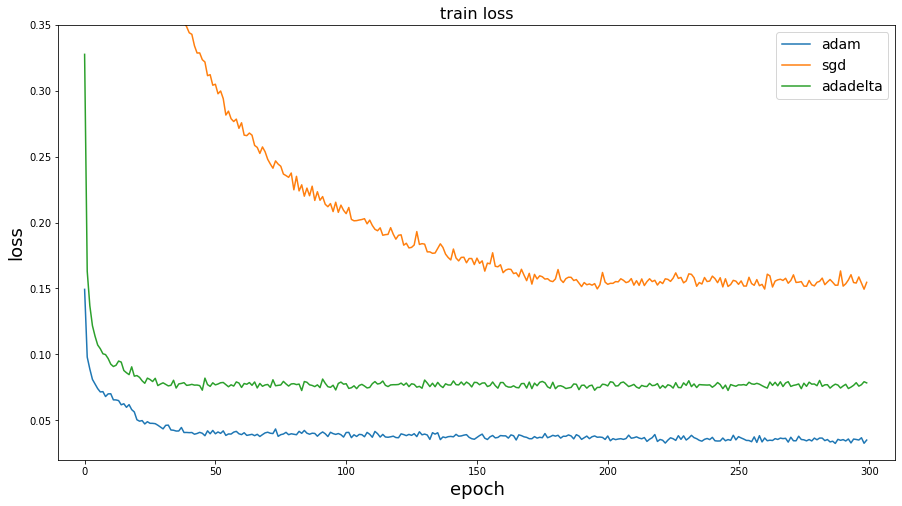
\includegraphics[width=.9\linewidth]{trainlos1.png}  
	\caption{Plot of the loss of the models after 300 epochs in the training dataset}
\label{fig5}
\end{figure}

\begin{figure}[]
  \centering
  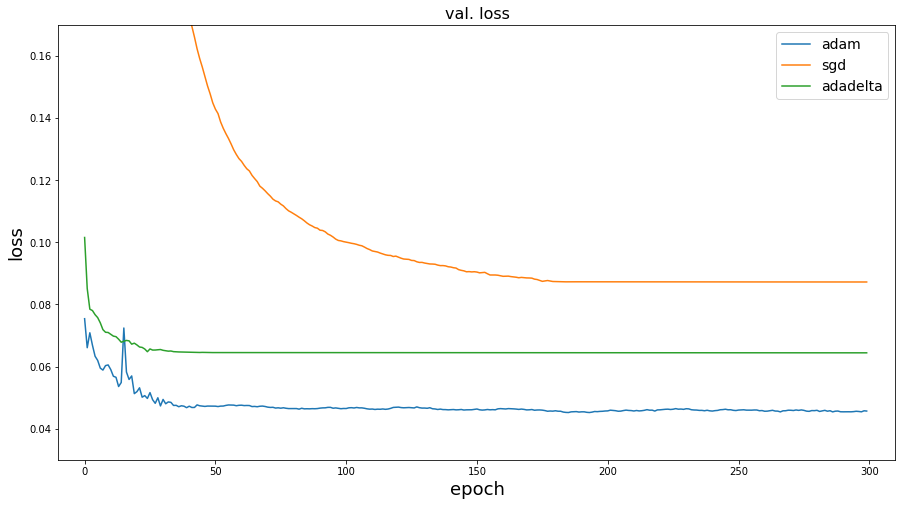
\includegraphics[width=.9\linewidth]{vallos1.png}  
	\caption{Plot of the loss of the models after 300 epochs in the validation dataset}
\label{fig6}
\end{figure}

\subsection{Experiments with SGD boosters}

In the Background section we mentioned that SGD is one of the oldest optimizers, so it is the more simple of all. That is why there are some boosters that improve the accuracy of the SGD optimizer. We mentioned them as momentum and Nesterov. In the case of Nesterov, in the code you only have to declare it as \textit{True} when you call for the SGD optimizer. In the case of the momentum, we used a 0.9 as its feature, even when it combines with Nesterov.\\

As we can see Figure \ref{fig7} and Figure \ref{fig8} we have the same parameters for SGD, Adam and Adadelta that we had in previous plots, and now we added the accuracy performance of the SGD optimizer with the different boosters. \\

In both cases, Adam is still the optimizer that reaches a higher accuracy percentage. But we also notice that all three of the SGD plus booster models are better than the Adadelta model. As we can see, the boosters help the SGD algorithm to reach a high accuracy in the first epochs, and then evens out the curve fairly quickly.\\

In Figure \ref{fig8} of the validation accuracy, we see however, that the spikes at the beginning of the line behave similar to the Adam optimizer, and same as Adam, in this plot, it reaches a lower accuracy than in training.\\

\begin{figure}[]
  \centering
  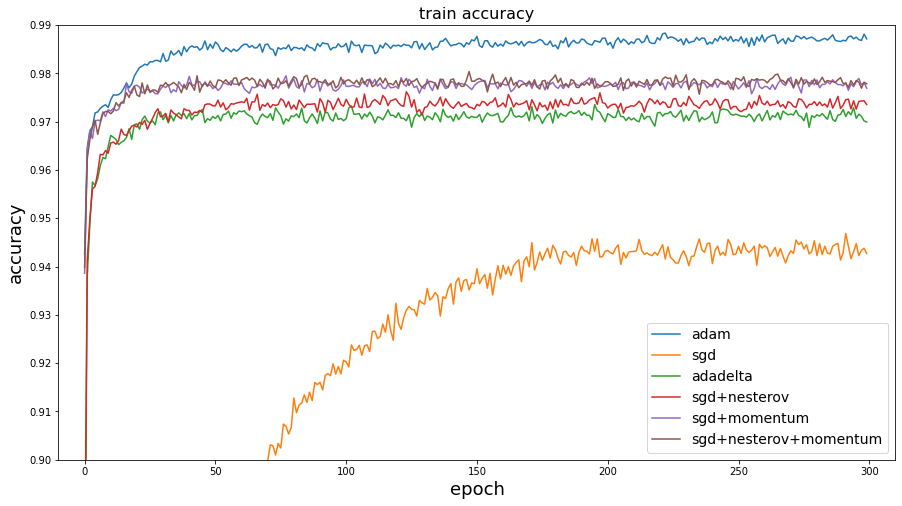
\includegraphics[width=.9\linewidth]{trainacc2.png}  
	\caption{Plot of the accuracy of the models after 300 epochs in the training dataset}
\label{fig7}
\end{figure}

\begin{figure}[]
  \centering
  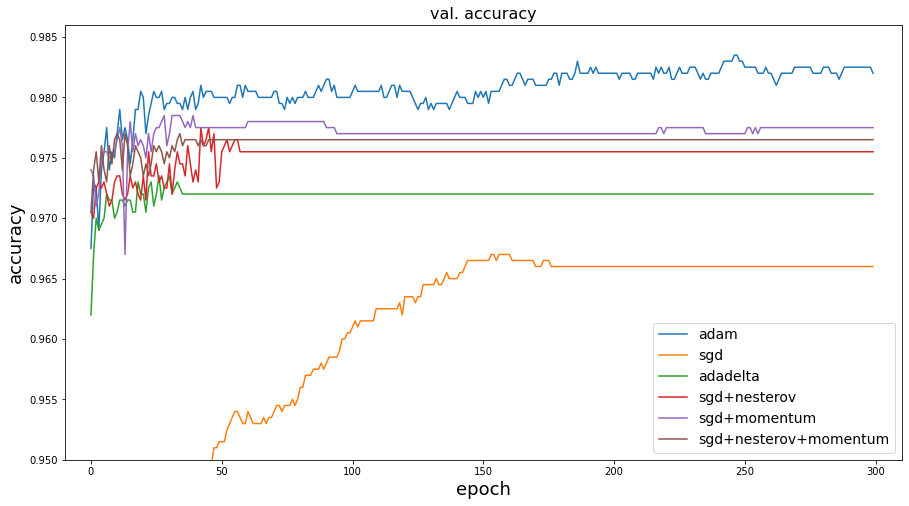
\includegraphics[width=.9\linewidth]{valacc2.png}  
	\caption{Plot of the accuracy of the models after 300 epochs in the validation dataset}
\label{fig8}
\end{figure}

For both loss plots in Figure \ref{fig9} and Figure \ref{fig10} we see a clear improvement in the loss rate, but same as with the accuracy plots, Adam keeps being the one with the best results.\\

\begin{figure}[]
  \centering
  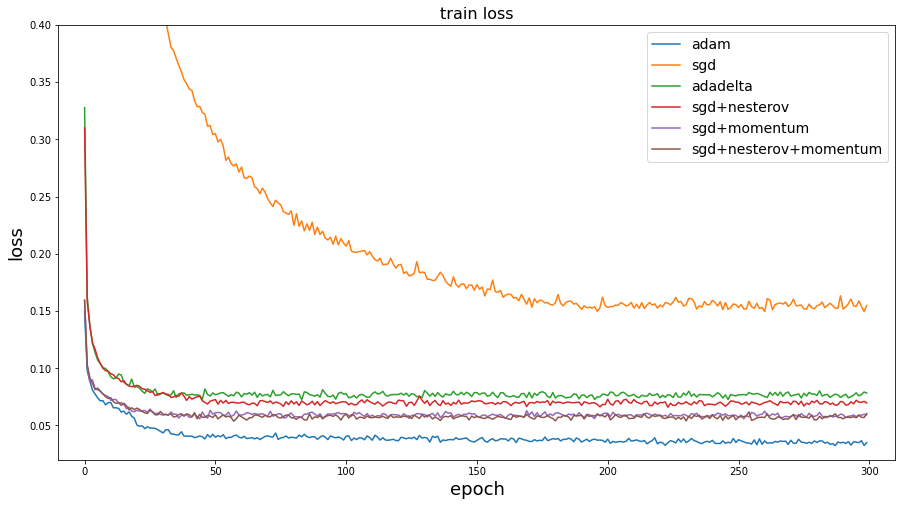
\includegraphics[width=.9\linewidth]{trainlos2.png}  
	\caption{Plot of the loss of the models after 300 epochs in the training dataset}
\label{fig9}
\end{figure}

\begin{figure}[]
  \centering
  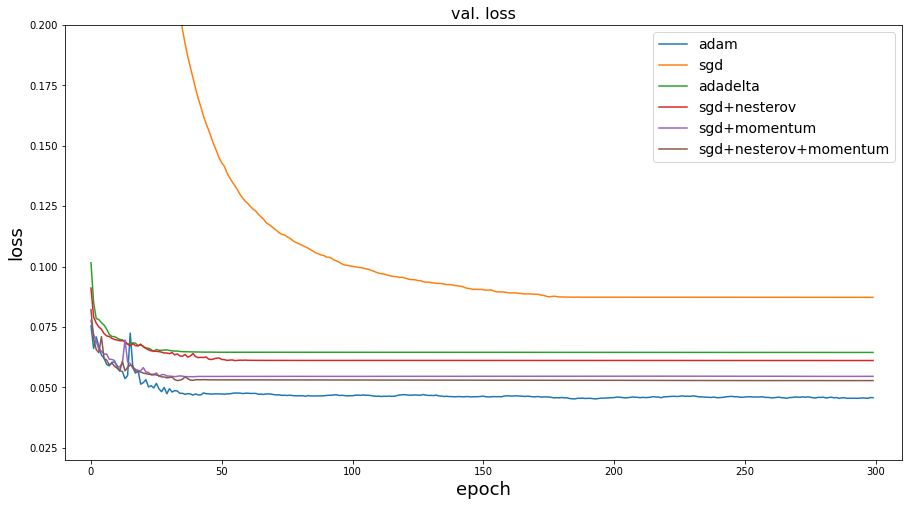
\includegraphics[width=.9\linewidth]{vallos2.png}  
	\caption{Plot of the loss of the models after 300 epochs in the validation dataset}
\label{fig10}
\end{figure}


\section{Conclusions and discussion}\label{conclusions}

We mentioned before that the main goal for this experimentation was to determine if improving the accuracy of our models was worth the computational processing and the time it would take to train more iterations to the CNN architectures we mentioned at the beginning. And the answer to that is no.\\

Thanks to the Law of large numbers we where able to identify that the average of the SGD optimizer compared to the others is not going to come close to their accuracy percentage in a feasible time.\\

In the case of SGD by its own, it is not feasible to give it so many iterations to have a result that we achieve with other optimizers easily. More if we take into consideration, that when we see the results when the slope finally evens out, the accuracy does not reach above of 96\% of accuracy. The boosters definitely helped improve the results of the SGD, but even so, Adam remains a better option than the boosters, given that they take way more time to compile.\\

The one optimizer that we were considering giving it more iterations because of its behaviors on the plot, was Adam, but when we finally compare the training plot with the validation plot, we see that there is a bit of a gap between the two, where the training performs way better than the validation set. \\

In the Methods and materials section we discussed the use of a restriction on the iterations, in which the epoch changes when the learning rate gets stuck after several iterations. This was thought out to avoid overfitting, which is what we think is happening with the Adam optimizer. Now, despite the restriction of the learning rate, we see signs of overfitting in the behavior of the training and validation sets of this optimizer, which is why, if we do experiment with only the Adam optimizer with our real images, we will not be using 300 epochs, and instead try at maximum 40 epochs, where we can see the curve of our model even out.\\

\section*{References}

\bibliography{Proyecto}

\end{document}